\chapter{Influential People Detection}
\label{chapter:influential people detection}

This chapter describes the process of detection of influential people from the people gazetteer developed in Chapter~\ref{chapter:people gazetteer} and its results with some case studies. Section~\ref{influential:rw} discusses some related work in the field of influential people detection, Section~\ref{influential:measure} the measures used to define an influential person in the newspaper environment followed by their ranking to obtain top influential persons across each person category with results in Section~\ref{influential:results} and some points of discussion in Section~\ref{influential:discussion}.

 
\section{Related Work}
\label{influential:rw}


Influential people detection has been mostly done in the field of social networks, marketing and diffusion research.
\cite{kempe2003maximizing} work on choosing the most influential set of nodes  in a social network in order to maximize user influence in the network. They consider spread of influence from an influential node cascading through a network which further influences other neighborhood nodes but we do not consider the case of a network of connected person entities in our research where influence score of a person entity could be influenced by that of its neighboring person entity nodes. We consider each person entity connected with a list of articles of its occurrence instead and measure the person entity's influence score by finding the effect of influence of each article in that list.
 

\cite{lerman2010using} define popularity of a news story in terms of number of reader votes received by it and predict popularity of a news story over time based on voting history and the probability that a user seeing a story at specific position in a list will vote on it. 
A more relevant work regarding detection of influential people is presented in \cite{agarwal2008identifying} where influential bloggers are identified on a blog site. Influence of each blogger is quantified by taking maximum of the influence scores of each blog posted by a blogger. The influence score of each blog is calculated using parameters of importance in a blogsite like number of posts that refer to the blog, number of comments on the blog, number of other posts that the blog refers to and length of the blog. Influential blogger categories are also created based on the temporal patterns of blog posting by bloggers. 

\cite{cha2010measuring} describe another set of measures for detection of top influential users on Twitter using number of retweets, mentions and followers for an individual. They perform ranking based on each measure separately and use Spearman's rank correlation coefficient to find correlation among ranks and effect of each measure contributing to a person's influence. The influence ranks of topmost influential users on Twitter are presented across various topics as well as time.

In the above mentioned works, although the problem description matches with our research problem but the parameters defined to measure influence or popularity cannot be directly used in the newspaper environment. 


\section{Measuring Influence}
\label{influential:measure}

To measure influence in the newspaper environment and to compare and rank people as influential, we define an influence score measure called \textit{``Influential Person Index" (IPI)} corresponding to each person entity in the people gazetteer. To calculate IPI for each person entity, we first define the \textit{``Document Index" (DI)} to measure how each document in the person entity's associated list of documents affects his influence score.
Following subsections describe the parameters for calculation of DI and IPI of a person entity followed by the complete algorithm for detection of influential persons:

\subsection{Document Index (DI)}

The Document Index (DI) of an article in the people gazetteer helps to measure a person's influence score. Following parameters are considered for the calculation of this index:

\begin{enumerate}
\item \textbf{Normalized Document Length} (NDL)\\
Document Length affects the influence score in the sense that a longer news article in which a person entity occurs is deemed to be more important than a shorter one. It is defined as the number of tokens contained in a news article. Document Length is further normalized by dividing it with the maximum news article length (of 14020 articles in the dataset) to get Normalized Document Length as follows: 

$$NDL=\dfrac{\text{Document Length}} {\text{Maximum Document Length in the dataset}}$$


%\item[$\bullet$IDF]
%IDF is used as a parameter in the calculation of DI of a news article to give weight to the person entity's occurrence in the complete %dataset. It can be calculated as the number of news articles in which a person entity occurs in the complete dataset. It is %equivalent to the length of document list in the people gazetteer for each person entity.

\item\textbf{ Normalized Term Frequency} (NTF)\\
Term Frequency (TF) accounts for the number of occurrences of a person's name in a news article. The TF of the person name affects a document's influence score as a higher number of occurrences in the document makes it more important. TF is further normalized and calculated as follows:

\begin{center}
$NTF=	1	+\log	$(TF of person entity in current article)
\end{center}

\item \textbf{Number of similar articles} (NSIM)\\
This parameter is used in calculation of the DI by finding articles of similar topic in the document list. 
%The set of topics derived from a corpus can be used to answer questions about the similarity of words and 
%documents.
Two documents are considered similar if they belong to the same topics. For a document $d$ whose DI is to be calculated, we consider 

SIM= Number of articles with the same topic as that of $d$ in the document list of person entity.

This measure is normalized by dividing it with the number of total articles in the document list of the person entity as follows:

\begin{center}
$NSIM= \dfrac{\text{SIM}} {\text{Total number of articles in the person's document list}}$
\end{center}
NSIM can be said to be equivalent to the proportion of topic similar articles that any document $d$ has.

This parameter takes into account the effect of a document's score on a person's IPI when there exist several other documents of the same topic in the person's list. 


\end{enumerate}

DI for each document is a function of the above mentioned parameters and is calculated using the following formula :
\begin{center}

			$DI = w_a . NDL + w_b . NSIM + w_c . NTF $
\end{center}
where, $w_a$,$ w_b$ and $w_c$ are the weights associated with each of the parameters NDL, NSIM and NTF respectively.


DI is actually a heuristic measure of these three parameters where each of the parameters can be weighted as per dataset characteristics and user requirements. For example, a higher value to $w_a$ and lower to $w_b$ and $w_c$ indicates documents with longer lengths are considered more important for influencing a person's IPI. On the other hand, a higher value to $w_b$ and lower to $w_a$ and $w_c$ indicates a document with larger proportion of topic similar articles influences the person's IPI more suggesting assignment of high influence score to a person entity occurring repeatedly in a specific news topic.  

\subsection{Influential Person Index (IPI)}

Once DI is calculated for each document in a person's list, an index is calculated for the person entity in order to measure its influence in the news dataset and calculate its influential score. The ``Influential Person Index" defined for this purpose is calculated as follows:
		
\begin{center}
$IPI= max DI(d_1, d_2, ...,d_n)+ UniqT$
\end{center}

where , $max DI(d_1, d_2, ...,d_n)$ = Maximum Document Index of a document $d_i$ in a person entity's list of  $n$ articles, and
\begin{center} $UniqT = \dfrac{\text{Number of Unique Article Topics in a person entity's document list}}{\text{Total Number of Topics in the corpus}}$\end{center} 

The parameter $UniqT$  is used to account for the fact that a single person entity can be talked about multiple news topics in the news articles and to include its effect on the person entity's influence score. It is normalized by dividing it with the total number of topics as obtained during topic detection on all 14020 articles.

Ranking is done across each person category of the people gazetteer to obtain top most influential persons. For this, IPI for each person entity across the person categories are sorted in decreasing order to obtain the most influential person entities with highest IPI at the top.
  
\subsection{Procedure for finding influential persons}

Algorithm ~\ref{algorithm:3} depicts the procedure for measuring influence and ranking of influential people from the gazetteer. It starts with calculation of DI for each news article in a person's document list by calculating the required parameters of NDL, NSIM and NTF which are assigned 0 values initially. The respective weights $w_a$,$w_b$,$w_c$ are taken as inputs and multiplied with each parameter to get final DI score which is added to the list of DI scores $DIScoreList$. The list is sorted to find the maximum DI value among all news articles in the person's document list. The maximum DI score is then added to the UniqT parameter to get the final IPI for each person entity which are again stored and sorted to obtain a ranked list of influential person entities.  

\begin{algorithm}[!htb]
\caption{Procedure to calculate IPI and rank person entities based on it}
\label{algorithm:3}
\begin{algorithmic}
\Function {CalculateIPI}{}
  


 \KwIn{$PeopleGazetter(Persons,(DocList,TopicList))$, $w_a$,$w_b$,$w_c$}
\KwResult{Ranked list of Person Name and IPI}  
 $NTF \leftarrow $0,  $NDL \leftarrow $0, $NSIM \leftarrow $0, $DI\leftarrow $0, $UniqT\leftarrow $0, $IPI\leftarrow $0\;  
  
    \For{(String PersonName : Persons)}
     {
	   \For{(String doc  : DocList)}
	{	
		$NTF=1+\log (GetPersonTF(doc))$;
		
$NDL=GetDocLength(doc)/GetMaxDocLength()$;

		$ NSIM=GetTopicSimilarArticles(doc,DocList)$;

		$DI=w_a . NDL+w_b . NSIM+ w_c . NTF$;
		
		$DIScoreList.add(DI)$;
 	 }
		$Sort(DIScoreList)$;

		$UniqT=GetUniqueTopics(Person,TopicList)$;

		$IPI=Max(DIScoreList)+UniqT$;

		$IPIScores.put(PersonName,IPI)$;
       }
	$Sort(IPIScores)$;

	$PrintPersonNameandMaxIPI(IPIScores)$;

\EndFunction

%\SetSideCommentLeft{$GetPersonTF(doc)$: calculates TF of person entity in document $doc$.

%$GetDocLength(doc)$: calculates number of tokens in $doc$.

% $GetMaxDocLength()$ : calculates maximum number of tokens in any document.

%$GetTopicSimilarArticles(doc,DocList)$: calculates normalized number of topic 

%similar articles for $doc$ in the $DocList$.

%$Sort(DIScoreList)$ :sorts the $DIScoreList$.

%$Max(DIScoreList)$ : finds the maximum score from $DIScoreList$.

%$GetUniqueTopics(Person,TopicList)$ : calculates normalized unique topics for

% $Person$ in its $TopicList$. 

%$Sort(IPIScores)$: sorts the $IPIScores$ by IPI values.

%$PrintPersonNameandMaxIPI(IPIScores)$ : prints $Person$ name with its IPI in decreasing order of IPI value. }	

\end{algorithmic}
\end{algorithm}

\begin{table}[h]
\begin{center}
\begin{tabular}{|c|c|} \hline
Function Name & Description \\ \hline
GetPersonTF(doc) & Calculates TF of the person entity \\
 & in document $doc$ \\ \hline
GetDocLength(doc) & Calculates number of tokens in $doc$. \\ \hline
GetMaxDocLength() & Calculates maximum number of \\
& tokens in any document.\\ \hline
GetTopicSimilarArticles(doc,DocList) &  Calculates normalized number \\
& of topic similar articles for $doc$ in the $DocList$. \\ \hline
Sort(DIScoreList) & Sorts the $DIScoreList$ \\ \hline
Max(DIScoreList) & Finds the maximum score from $DIScoreList$. \\ \hline
GetUniqueTopics(Person,TopicList) & Calculates normalized unique \\
& topics for $Person$ in its $TopicList$. \\ \hline
Sort(IPIScores) & Sorts the $IPIScores$ by IPI values. \\ \hline
PrintPersonNameandMaxIPI(IPIScores) & Prints $Person$ name with its \\
& IPI in decreasing order of IPI value. \\ \hline
\end{tabular}
\end{center}
\caption{Description of the functions used in Algorithm~\ref{algorithm:3}}
\label{default}
\end{table}%

\begin{figure}[h]
\begin{center}
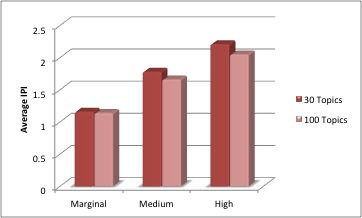
\includegraphics[scale=0.75]{IPIChart}
\end{center}
%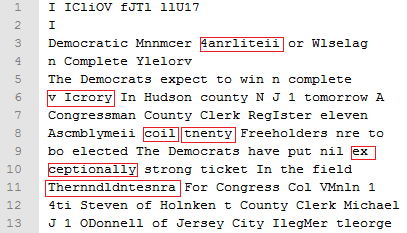
\includegraphics[scale=0.80]{ocr}
\caption{Comparison of the Average IPI for two ranked lists $L_1$ and $L_2$ using $30$ and $100$ topics respectively.}
\label{figure:IPI}
\end{figure}


%\newpage
\section{Results}
\label{influential:results}
Two ranked influential person lists, namely L1 and L2 are obtained after calculation of IPI from the people gazetteer (developed in Chapter~\ref{chapter:people gazetteer}) using 30 Topics and 100 Topics LDA Model respectively. The weights $w_a$, $w_b$ and $w_c$ are all set to 1 to give equal importance to each of the parameters during calculation of DI and IPI. The statistics obtained from both lists with respect to each person category of the people gazetteer are shown in Table~\ref{table:stats}. 
It can be clearly observed from the table that Highly Influential Persons occur in most number of news articles on an average and with highest average term frequency followed by Medium Influential and Marginal Influential Persons.
Document Length need not always be too high for a person to be ranked higher as can be observed from the fact that average document length obtained for Marginally Influential People is high in spite of their Average IPI being low indicating that the varying number of similar articles for each document as well as its Term Frequency share also play an important part in measuring influence. Figure~\ref{figure:IPI} shows the average IPI from the two ranked lists -- it appears that the average IPI for highly influential people is more susceptible to changes in number of topics.



%\begin{table}
%\begin{center}

%    \begin{tabular}{|p{2cm}|p{2cm}|p{2cm}|p{2cm}|p{2cm}|p{2cm}|p{2cm}|}
%    \hline
%    \textbf{Person Category}  &  \textbf{Number of Person Entities}   & \textbf{Average Number of Documents}   &  \textbf{Average Document Length}	&  \textbf{Average Term Frequency}	&	\textbf{Average IPI(List 1)} & \textbf{Average IPI(List 2)}\\  \hline
%Marginal & 38066 & 1.04 & 2119.6 & 1.07 & 1.16	& 1.14	\\ \hline
%Medium & 344 & 5.75 & 1976.3 & 6.68 & 1.78 & 1.66	 \\ \hline
%High & 16 & 22.8 & 2971.5 & 29.870	& 2.21 &	2.05	 \\	\hline 
%  \end{tabular}
%  \end{center}
%    \caption {Table illustrating average statistics for each Person Category of People Gazetteer across 2 Topic Models}
%\label{table:stats}
%\end{table}

\begin{table}
\begin{center}

    \begin{tabular}{|p{2cm}|p{2cm}|p{2cm}|p{2cm}|p{2cm}|}
    \hline
    \textbf{Person Category}  &  \textbf{Number of Person Entities}   & \textbf{Average Number of Documents}   &  \textbf{Average Document Length}	&  \textbf{Average Term Frequency}	\\  \hline
Marginal & 38066 & 1.04 & 2119.6 & 1.07 	\\ \hline
Medium & 344 & 5.75 & 1976.3 & 6.68  \\ \hline
High & 16 & 22.8 & 2971.5 & 29.870	 \\	\hline 
  \end{tabular}
  \end{center}
    \caption {Table illustrating average statistics for each Person Category of People Gazetteer across 2 Topic Models}
\label{table:stats}
\end{table}


The following sections present comparison between the ranked influential person lists L1 and L2, some case studies and evaluation results:
 
\begin{table}[!h]
\begin{tabular}{|p{2cm}|l|p{1.5cm}|p{1.5cm}|l|l|l|p{3cm}|l|l|}
\hline
Person Name    & IPI  & Number of Articles & Person Category & NDL  & NTF  & NSIM & TOPIC WORDS                                                          & UniqT & Rank \\ \hline
capt creeten   & 3.38 & 10                 & Medium          & 0.56 & 1.95 & 0.8  & mr court police judge justice case yesterday street district         & 0.06  & 1    \\ \hline
capt hankey    & 3.02 & 6                  & Medium          & 0.68 & 1.6  & 0.66 & club game team play football half ball left college back             & 0.06  & 2    \\ \hline
capt pinckney  & 2.93 & 3                  & Marginal        & 0.38 & 1.84 & 0.67 & man ho men night back wa room left house told bad                    & 0.03  & 3    \\ \hline
john macdonald & 2.85 & 3                  & Marginal        & 0.55 & 2.2  & 0    & great people life man women good country world american part         & 0.1   & 4    \\ \hline
john martin    & 2.82 & 12                 & Medium          & 0.56 & 1.6  & 0.5  & mr court police judge justice case yesterday street district witness & 0.17  & 5    \\ \hline
aaron trow     & 2.81 & 1                  & Marginal        & 0.7  & 2.07 & 0    & man ho men night back wa room left house told                        & 0.03  & 6    \\ \hline
mrs oakes      & 2.79 & 5                  & Medium          & 0.08 & 2.04 & 0.6  & street mrs mr avenue wife house miss yesterday years home            & 0.06  & 7    \\ \hline
buenos ayres   & 2.76 & 6                  & Medium          & 0.43 & 1.6  & 0.67 & white water indian black long found thu big dog time                 & 0.06  & 8    \\ \hline
alexander iii  & 2.74 & 31                 & High            & 0.24 & 2.04 & 0.29 & great people life man women good country world american part         & 0.16  & 9    \\ \hline
mr got         & 2.73 & 3                  & Marginal        & 0.56 & 1.47 & 0.67 & mr court police judge justice case yesterday street district witness & 0.03  & 10    \\ \hline
\end{tabular}
\caption{Table showing top 10 influential persons of List L1 detected from People Gazetteer with 30 Topics LDA model. Parameters NDL, NTF,NSIM and Topic Words belong to the maximum scoring DI in the person's document list.}
\label{table:30t}
\end{table}

\begin{table}[!h]
\resizebox{16cm}{!} {
\begin{tabular}{|p{2cm}|l|p{1.5cm}|p{1.5cm}|l|l|l|p{3cm}|l|l|}
\hline
Person Name    & IPI  & Number of Articles & Person Category        & NDL  & NTF  & NSIM & Topic Words                                                                 & UniqT & Rank \\ \hline
capt creeten   & 3.33 & 10                 & Medium     & 0.56 & 1.95 & 0.8  & mr police witness committee capt asked captain money inspector paid         & 0.02  & 1    \\ \hline
mrs martin     & 3.23 & 8                  & Medium     & 0.20 & 2.38 & 0.5  & mrs mr years wife home house ago woman city died                            & 0.02  & 2    \\ \hline
alexander iii  & 3.09 & 31                 & High     & 0.49 & 2.04 & 0.48 & emperor prince french alexander czar london nov government imperial russian & 0.07  & 3    \\ \hline
capt hankey    & 2.97 & 6                  & Medium    & 0.68 & 1.6  & 0.66 & game team football play half line ball back yale eleven                     & 0.02  & 4    \\ \hline
aaron trow     & 2.79 & 1                  & Marginal & 0.70 & 2.07 & 0    & day place long great water time feet found good men                         & 0.01  & 5    \\ \hline
john macdonald & 2.77 & 3                  & Marginal & 0.55 & 2.2  & 0    & people american man great country men world life good english               & 0.02  & 6    \\ \hline
mrs oakes      & 2.74 & 5                  & Medium     & 0.08 & 2.04 & 0.6  & mrs mr years wife home house ago woman city died                            & 0.02  & 7    \\ \hline
john martin    & 2.71 & 12                 & Medium     & 0.56 & 1.6  & 0.5  & mr police witness committee capt asked captain money inspector paid         & 0.05  & 8    \\ \hline
ed kearney     & 2.63 & 7                  & Medium     & 0.16 & 1.6  & 0.85 & won time race ran mile furlough half lo track fourth                        & 0.01  & 9    \\ \hline
caleb morton   & 2.61 & 1                  & Marginal & 0.70 & 1.9  & 0    & day place long great water time feet found good men                         & 0.01  & 10   \\ \hline

\end{tabular}}
\caption{Table showing top 10 influential persons of  List L2 detected from People Gazetteer with 100 Topics LDA model. Parameters NDL, NTF,NSIM and Topic Words belong to the maximum scoring DI in the person's document list.}
\label{table:100t}
\end{table}
\subsection{Comparison Across Ranked Influential Person Lists }

The top 10 influential persons from List L1 and L2 detected from each of the people gazetteers are presented in Table ~\ref{table:30t} and ~\ref{table:100t} respectively.
It can be clearly seen from both the tables that the person category labels assigned during development of people gazetteer do not hold true after detection of influential persons. This suggests that the highly influential category people which were defined as person entities with more than 16 articles in the dataset might not necessarily be the most influential. The top 10 influential persons in both tables are dominated by Medium and Marginal category persons having considerably less number of articles of occurrence. This indicates the fact that number of articles of occurrence has not been given priority while measuring influence of a person entity. 
The statistics for top 10 influential people from both the tables also suggest that none of the measures of NDL, NTF or NSIM can be alone used to say whether a person entity is influential since these value do not decrease or increase consistently although the NTF measure does contribute most to the IPI of any person.

\newpage
The ranked influential lists L1 and L2 can be contrasted in terms of NSIM, UniqT and Topic Words since they vary across different number of topics and to see the effect of 30 and 100 Topics LDA Models on influential person detection.
 If NSIM (normalized number of topic similar articles) remains same in L1 and L2 during influential person detection from both the people gazetteers, then the same highest scoring article' DI is selected for calculation of IPI in both of them. This is why the parameters NDL (Normalized Document Length) and NTF (Normalized Term Frequency) remain same across both the lists. This can be seen for person like ``capt creeten", ``capt hankey", ``aaron trow" and "mrs oakes" in Tables ~\ref{table:30t} and ~\ref{table:100t}. But the value of UniqT for these persons decreases leading to decrease in their final IPI in the second table. This is because LDA model with higher number of topics (100) is used in this case due to which the proportion of unique topics becomes lower when NSIM does not change.
However, when the NSIM (normalized number of topic similar articles) value changes because of change in number of topics, a different article with maximum DI score can get selected leading to change in the values of NDL, NTF, UniqT and the final IPI. This causes a shift in the ranking of influential persons across the two lists and can be seen when the rank of ``alexander iii" in the first table moves from 9 to 3 in the second table. 
This indicates the fact that LDA Topic Model used affects the ranking of influential persons when number of topics are varied.

  \subsection{Case Studies}

Some of the topmost 10 influential person entities of lists L1 and L2  (Table ~\ref{table:30t} and ~\ref{table:100t}) identified from each person category of the 2 people gazetteers are discussed below: 
\begin{enumerate}

\item
Highly Influential Category- This category as defined in Section~\ref{ner:results} includes person entities influencing number of news articles greater than 16. However, only one person entity (``alexander iii") from this category occurs in the top 10 influential persons. The entry for ``alexander iii" has an IPI of 2.94 and 3.09 respectively in list L1 and L2 . The person entity occurs in 31 news articles with 5 and 7 different topics in each of the lists. The most common topic words associated with this person entity are: ``emperor prince french alexander czar london nov government imperial russian" indicating the importance of this entity in government related news topics. The 100 Topic LDA model increases the IPI value of this entity because the NSIM value increases (more number of similar topic articles talk about this person) and a longer article gets maximum DI score resulting in a high IPI value and improvement in the ranking from rank 9 in the first table to rank 3 in the second.

\item
Medium Influential Category- The top 10 influential entities from Tables ~\ref{table:30t} and ~\ref{table:100t} contain the most number of person entities from this person category. The person entity``capt creeten" has been ranked as highest influential (Rank 1) across both the tables. It occurs in 10 news articles with 9 of them belonging to the same topic indicating the person influencing news articles of high topic similarity. Some of the most common topic words for this entity include `` mr police witness committee capt asked captain money inspector paid" indicating the importance of this entity in a judicial or police related news topic.
Several persons from this category like ``mrs martin" , ``mrs oakes"  although identified among the top 10 influential persons but suffer from the problem of co-referred person names and named entity disambiguation as it is hard to identify which exact person they refer to due to lack of first names.
 
\item
Marginally Influential Category- Person entities belonging to this category have extremely low occurrence in news articles although the IPI of topmost influential entities belonging to this category are comparable to those in the other 2 categories.
Several person entities with low occurrences in news articles like ``aaron trow", ``caleb morton", ``john macdonald"  belong to this category. These entities in spite of occurring in very few articles (1 to 3) occur a large number of times in those articles with comparatively longer article length indicating the importance of these entities with respect to the articles they occur in. Since each of the features has been given equal weight during the calculation of IPI,  these person entities with high NDL and NTF have been identified among the top 10 influential persons. 
 The person entity ``mr got" ranked as a high influential person belonging to this category has actually been falsely detected as influential as the PNER seems to have misrecognized this entity as a person entity.  

\end{enumerate} 


\subsection{Evaluation}

Due to the unavailability of ground truth consisting of influential people in the newspaper archives from November-December 1894, there is no way to validate our results. 
To broadly evaluate our results, a simple web search query with the person entity's name in the context of 19th century was done on the Wikipedia website for the top 30 influential persons of Lists L1 and L2 detected from the people gazetteer with 30 Topics LDA and 100 Topics LDA Model respectively.

Among the top 30, 16 person entities from List L1 and 14 from List L2 were found to be influential and popular in the 19th century across topic categories like theatre, politics, government, shipping, etc. Some of these influential persons from Lists L1 and L2 found in Wikipedia are shown in Figure~\ref{figure:inf}. 

\begin{figure}[!htb]
\begin{center}
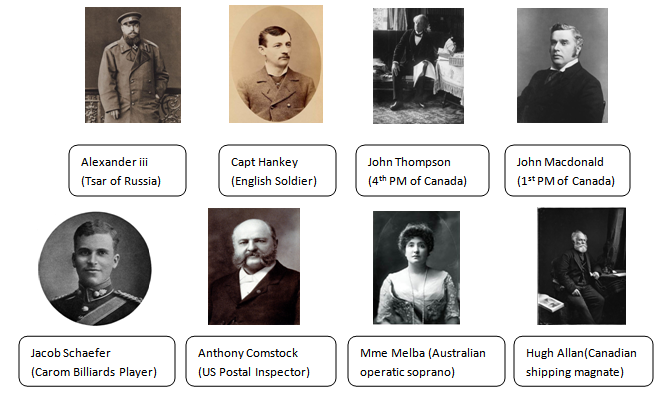
\includegraphics[scale=0.79]{ip}
\caption{Some of the top 30 influential persons obtained from the dataset and also found on Wikipedia during evaluation}
\label{figure:inf}
\end{center}
\end{figure}


 Most of the false positives although influential in other respects but were not  influential `person' entities which can attributed to the incorrect PNER (Person Named Entity Recognition) on noisy OCR data.
 False positives are obtained for person entities  such as ``mr got" which is not a person entity at all and for entities such as ``ann arbor" and ``van cortlandt" which are in fact locations but got recognized as highly influential person entities.
 
 The ranked list of the top 30 influential persons with their IPI from Lists L1 and L2 can be seen in the Appendix (Table ~\ref{table:app1}.~\ref{table:app2}) where evaluation result for each person entity is also presented.


\section{Discussion}
\label{influential:discussion}


\begin{description}
\item[$\bullet$]\noindent
We used a linear combination of each of the parameters in calculation of DI and IPI and assigned equal values to the weights associated with each of them by not favoring any specific parameter. This is evident from the results which do not consistently favor any specific parameter. The parameters defined are based on heuristics and can be re-weighted according to user requirements or new parameters can be defined to do so. 

\item[$\bullet$]\noindent
The parameters for calculation of DI and IPI can also be learned by performing regression analysis using a manually developed sample of topmost influential people and obtaining the complete list of ranked influential people based on the learned parameters.

\item[$\bullet$]\noindent
The NDL(Normalized Document Length) parameter defined for calculation of DI is normalized using the maximum length of any document in the dataset. However, there might exist other ways of normalization of Document Length like using total number of tokens in a person entity's document list or total number of tokens in the complete dataset which can be experimented with according to the dataset.

\item[$\bullet$]\noindent
The topmost influential people contain several false positives also which occur not due to the influence measures defined but due to other factors discussed in Section ~\ref{gaz:discussion}. Several location and organization names have been misrecognized as person entities after performing Spelling correction and PNER resulting in false detection of some highly influential entities like ``van cortlandt", ``ann arbor" , ``sandy hook", etc.  There is also the problem of resolution of person name co-references in cases where persons like ``mrs martins" , ``mrs oakes", etc. have been recognized as influential.  

\item[$\bullet$] \noindent
The choice of parameters for topic detection also affects the detection of influential people which is evident from the fact that we get different ranking of influential people for the two different LDA Topic model settings used. 

\end{description}